\documentclass[10pt,twocolumn]{article}
\usepackage[margin=0.75in]{geometry}
\usepackage{amsmath,amssymb,amsfonts}
\usepackage{graphicx}
\usepackage{booktabs}
\usepackage{hyperref}
\usepackage{xcolor}
\usepackage{tikz}
\usetikzlibrary{shapes,arrows.meta,positioning,fit,backgrounds,calc}
\usepackage{algorithm}
\usepackage{algorithmic}
\usepackage[font=small]{caption}
\usepackage{enumitem}

\setlength{\parskip}{0pt}

\title{\vspace{-1.5em}\textbf{Method: Hierarchical Residual Quantization with\\Language-Guided Codebook Learning for Sign Language Generation}}
\author{}
\date{}

\begin{document}
\maketitle
\vspace{-2em}

\section{Overview}

We present a two-stage framework for text-conditioned sign language motion generation. Given an input text description, our goal is to synthesize realistic full-body signing motion represented as SMPL-X pose parameters. Our approach decomposes the problem into (1)~learning a compact discrete motion representation via a \emph{Language-Guided Residual Vector Quantized Variational Autoencoder} (LG-RVQ-VAE), and (2)~modeling the conditional distribution over this discrete space using a \emph{Hierarchical Autoregressive Transformer}. Figure~\ref{fig:overview} illustrates the overall pipeline.

\begin{figure*}[t]
\centering
\resizebox{\textwidth}{!}{%
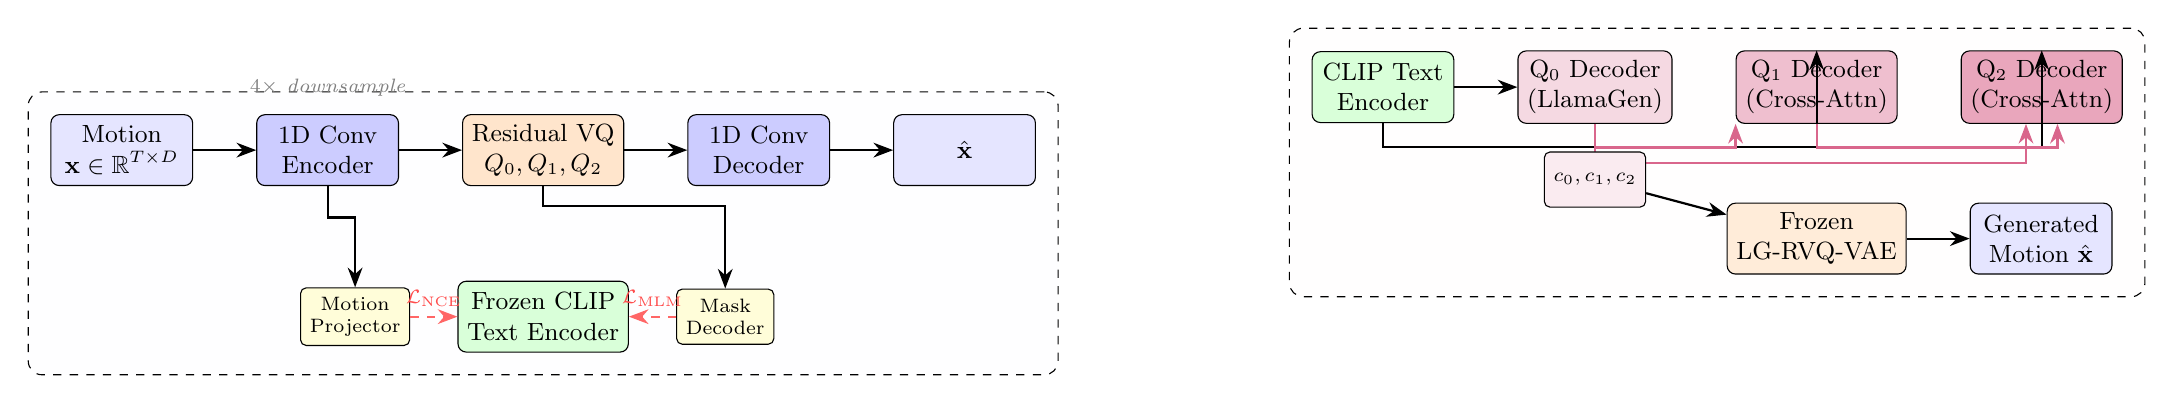
\begin{tikzpicture}[
    node distance=0.6cm and 0.8cm,
    block/.style={rectangle, draw, rounded corners=3pt, minimum height=0.9cm, minimum width=1.8cm, align=center, font=\small},
    smallblock/.style={rectangle, draw, rounded corners=2pt, minimum height=0.7cm, minimum width=1.2cm, align=center, font=\scriptsize},
    arrow/.style={-{Stealth[length=2.5mm]}, thick},
    dasharrow/.style={-{Stealth[length=2.5mm]}, thick, dashed},
    label/.style={font=\scriptsize\itshape, text=gray},
    stagebox/.style={draw, dashed, rounded corners=5pt, inner sep=8pt, fill opacity=0.05},
]

% === STAGE 1 ===
\node[block, fill=blue!10] (motion) {Motion\\$\mathbf{x} \in \mathbb{R}^{T \times D}$};
\node[block, fill=blue!20, right=of motion] (enc) {1D Conv\\Encoder};
\node[block, fill=orange!20, right=of enc] (rvq) {Residual VQ\\$Q_0, Q_1, Q_2$};
\node[block, fill=blue!20, right=of rvq] (dec) {1D Conv\\Decoder};
\node[block, fill=blue!10, right=of dec] (recon) {$\hat{\mathbf{x}}$};

\node[block, fill=green!15, below=1.2cm of rvq] (clip) {Frozen CLIP\\Text Encoder};
\node[smallblock, fill=yellow!15, left=0.6cm of clip] (proj) {Motion\\Projector};
\node[smallblock, fill=yellow!15, right=0.6cm of clip] (mask) {Mask\\Decoder};

\draw[arrow] (motion) -- (enc);
\draw[arrow] (enc) -- (rvq);
\draw[arrow] (rvq) -- (dec);
\draw[arrow] (dec) -- (recon);

\draw[arrow] (enc.south) -- ++(0,-0.4) -| (proj.north);
\draw[arrow] (rvq.south) -- ++(0,-0.25) -| (mask.north);
\draw[dasharrow, color=red!60] (proj.east) -- (clip.west) node[midway, above, font=\scriptsize, color=red!70] {$\mathcal{L}_{\text{NCE}}$};
\draw[dasharrow, color=red!60] (mask.west) -- (clip.east) node[midway, above, font=\scriptsize, color=red!70] {$\mathcal{L}_{\text{MLM}}$};

\node[label, above=0.1cm of enc] {$4\times$ downsample};

\begin{scope}[on background layer]
    \node[stagebox, fill=blue!5, fit=(motion)(enc)(rvq)(dec)(recon)(proj)(clip)(mask), label={[font=\small\bfseries]above:Stage 1: Language-Guided RVQ-VAE}] {};
\end{scope}

% === STAGE 2 ===
\node[block, fill=green!15, right=3.5cm of recon, yshift=0.8cm] (text2) {CLIP Text\\Encoder};
\node[block, fill=purple!15, right=0.8cm of text2] (q0dec) {Q$_0$ Decoder\\(LlamaGen)};
\node[block, fill=purple!25, right=0.8cm of q0dec] (q1dec) {Q$_1$ Decoder\\(Cross-Attn)};
\node[block, fill=purple!35, right=0.8cm of q1dec] (q2dec) {Q$_2$ Decoder\\(Cross-Attn)};

\node[block, fill=orange!15, below=1.0cm of q1dec] (frozen) {Frozen\\LG-RVQ-VAE};
\node[block, fill=blue!10, right=0.8cm of frozen] (output) {Generated\\Motion $\hat{\mathbf{x}}$};

\draw[arrow] (text2) -- (q0dec);
\draw[arrow] (text2.south) -- ++(0,-0.3) -| (q1dec.north);
\draw[arrow] (text2.south) -- ++(0,-0.3) -| (q2dec.north);
\draw[arrow, color=purple!60] (q0dec.south) -- ++(0,-0.3) -| (q1dec.south west);
\draw[arrow, color=purple!60] (q0dec.south) -- ++(0,-0.5) -| ([xshift=-0.2cm]q2dec.south);
\draw[arrow, color=purple!60] (q1dec.south) -- ++(0,-0.3) -| ([xshift=0.2cm]q2dec.south);

\node[smallblock, fill=purple!8, below=0.35cm of q0dec] (codes) {$c_0, c_1, c_2$};
\draw[arrow] (codes) -- (frozen);
\draw[arrow] (frozen) -- (output);

\begin{scope}[on background layer]
    \node[stagebox, fill=purple!5, fit=(text2)(q0dec)(q1dec)(q2dec)(frozen)(output)(codes), label={[font=\small\bfseries]above:Stage 2: Hierarchical Autoregressive Transformer}] {};
\end{scope}

\end{tikzpicture}
}%
\caption{\textbf{Method Overview.} \textbf{Stage~1} trains an LG-RVQ-VAE that learns language-aligned discrete motion codes via reconstruction and cross-modal alignment losses. \textbf{Stage~2} trains a hierarchical autoregressive transformer that generates motion codes conditioned on text, with each quantizer level refining the previous.}
\label{fig:overview}
\end{figure*}

\section{Stage 1: Language-Guided RVQ-VAE}
\label{sec:stage1}

\subsection{Residual Vector Quantized Autoencoder}

We encode continuous motion sequences $\mathbf{x} \in \mathbb{R}^{T \times D}$ (where $D{=}133$ represents upper-body SMPL-X parameters) into a compact discrete representation using a residual vector quantization scheme.

\paragraph{Encoder.} The encoder $E$ consists of a stack of strided 1D convolutional layers interleaved with residual blocks using dilated convolutions (dilation growth rate $r{=}3$, depth $d{=}3$). With downsampling factor $2$ applied across $2$ stages, the encoder achieves $4\times$ temporal compression:
\begin{equation}
    \mathbf{z} = E(\mathbf{x}) \in \mathbb{R}^{T' \times C}, \quad T' = T/4,
\end{equation}
where $C{=}512$ is the latent dimension.

\paragraph{Residual Vector Quantization.} Rather than using a single codebook, we employ Residual Vector Quantization (RVQ)~\cite{soundstream} with $K{=}3$ quantization stages. Each stage $k$ quantizes the residual from all previous stages:
\begin{align}
    \mathbf{r}_0 &= \mathbf{z}, \\
    c_k(t) &= \arg\min_{j} \| \mathbf{r}_k(t) - \mathbf{e}_k^j \|_2, \\
    \mathbf{r}_{k+1}(t) &= \mathbf{r}_k(t) - \mathbf{e}_k^{c_k(t)},
\end{align}
where $\mathbf{e}_k^j \in \mathbb{R}^{C}$ is the $j$-th entry in the $k$-th codebook of size $N{=}512$, and $c_k(t) \in \{0, \ldots, N{-}1\}$ is the discrete code at timestep $t$. The quantized representation is the sum of all selected codewords:
\begin{equation}
    \hat{\mathbf{z}}(t) = \sum_{k=0}^{K-1} \mathbf{e}_k^{c_k(t)}.
\end{equation}
Codebooks are updated via exponential moving average (EMA) with periodic reset of underutilized codes. During training, we apply \emph{quantizer dropout} with probability $p{=}0.2$, randomly using fewer than $K$ quantizers. This encourages earlier quantizers to carry more information and improves robustness at inference when using partial codebooks.

\paragraph{Decoder.} The decoder $G$ mirrors the encoder with transposed convolutions for upsampling and reconstructs the motion: $\hat{\mathbf{x}} = G(\hat{\mathbf{z}}) \in \mathbb{R}^{T \times D}$.

\subsection{Language-Guided Codebook Learning}

A key challenge in motion tokenization is ensuring that the learned discrete codes capture semantically meaningful structure rather than only low-level kinematic details. We address this by introducing three cross-modal alignment objectives that leverage a frozen CLIP text encoder to inject linguistic supervision into the codebook learning process.

\paragraph{Global Contrastive Alignment (InfoNCE).}
We project mean-pooled encoder features to the CLIP text space via a learnable projector $f_\theta$:
\begin{equation}
    \mathbf{v} = f_\theta\!\left(\frac{1}{T'}\sum_{t} \mathbf{z}(t)\right) \in \mathbb{R}^{d_\text{text}},
\end{equation}
and align them with the CLIP [EOS] text embedding $\mathbf{t}$ via InfoNCE:
\begin{equation}
    \mathcal{L}_{\text{NCE}} = -\frac{1}{B}\sum_{i=1}^{B} \log \frac{\exp(\mathbf{v}_i^\top \mathbf{t}_i / \tau)}{\sum_{j=1}^{B} \exp(\mathbf{v}_i^\top \mathbf{t}_j / \tau)},
\end{equation}
where $\tau{=}0.07$ is the temperature and $B$ is the batch size (with negatives gathered across GPUs in distributed training).

\paragraph{Masked Text Prediction.}
To encourage fine-grained token-level alignment, we randomly mask ${\sim}15\%$ of CLIP text tokens and train a lightweight decoder (2-layer transformer with cross-attention to motion tokens) to reconstruct the masked tokens:
\begin{equation}
    \mathcal{L}_{\text{MLM}} = -\sum_{m \in \mathcal{M}} \log p(w_m \mid \mathbf{w}_{\backslash \mathcal{M}}, \hat{\mathbf{z}}),
\end{equation}
where $\mathcal{M}$ is the set of masked positions and $w_m$ are the ground-truth CLIP vocabulary tokens. We apply label smoothing ($\epsilon{=}0.1$).

\paragraph{Weighted Relation Supervision (WRS).}
Beyond point-wise alignment, we enforce structural consistency between the pairwise similarity matrices of text and motion token representations:
\begin{equation}
    \mathcal{L}_{\text{WRS}} = \| \mathbf{S}_\text{text} - \mathbf{S}_\text{motion} \|_F^2,
\end{equation}
where $\mathbf{S}_\text{text}$ and $\mathbf{S}_\text{motion}$ are cosine similarity matrices computed over text tokens and their nearest-neighbor motion token projections, respectively.

\paragraph{Total Stage~1 Loss.}
The overall training objective combines reconstruction, commitment, and language-guided losses:
\begin{equation}
    \mathcal{L}_{\text{S1}} = \underbrace{\mathcal{L}_{\text{recon}}}_{\text{L1-smooth}} + \lambda_c \underbrace{\mathcal{L}_{\text{commit}}}_{\text{VQ}} + \lambda_l \big(\alpha \mathcal{L}_{\text{NCE}} + \beta \mathcal{L}_{\text{MLM}} + \gamma \mathcal{L}_{\text{WRS}}\big),
    \label{eq:stage1_loss}
\end{equation}
where $\lambda_c{=}0.25$, $\lambda_l{=}0.01$, $\alpha{=}0.001$, $\beta{=}0.01$, $\gamma{=}0.0001$.

\section{Stage 2: Hierarchical Autoregressive Transformer}
\label{sec:stage2}

With the frozen LG-RVQ-VAE providing semantically grounded motion tokens, we train a hierarchical autoregressive model to generate motion codes conditioned on text input. The key insight is that the RVQ structure naturally induces a coarse-to-fine hierarchy: $Q_0$ captures the dominant motion structure while $Q_1$ and $Q_2$ progressively refine details. We exploit this hierarchy with three specialized decoders.

\subsection{Architecture}

\paragraph{Text Conditioning.}
Input text is encoded by a frozen CLIP encoder into a sequence of features $\mathbf{h}_\text{text} \in \mathbb{R}^{S \times d_\text{text}}$, which are projected to the model dimension $d{=}1024$ via a learned linear layer.

\paragraph{Q$_0$ Decoder (Coarse).}
The coarse decoder models $p(c_0^{1:T'} \mid \text{text})$ autoregressively. We adopt a LlamaGen-style architecture with:
\begin{itemize}[nosep,leftmargin=*]
    \item \textbf{RMSNorm} pre-normalization for training stability,
    \item \textbf{Grouped Query Attention} (GQA) for memory efficiency,
    \item \textbf{SwiGLU} feed-forward layers,
    \item \textbf{1D Rotary Position Embeddings} (RoPE) for positional encoding,
    \item \textbf{Prefix concatenation}: text tokens are prepended to the motion sequence as a conditioning prefix (with zero-rotation RoPE for prefix positions).
\end{itemize}
The decoder consists of 9 transformer blocks with 16 attention heads. An output head projects to $N{+}1$ logits (512 motion codes + 1 \texttt{EOS} token for learned length control).

\paragraph{Q$_1$ Decoder (Medium Refinement).}
The Q$_1$ decoder models $p(c_1^{1:T'} \mid c_0^{1:T'}, \text{text})$ with a standard transformer architecture augmented with two cross-attention mechanisms:
\begin{itemize}[nosep,leftmargin=*]
    \item \textbf{Text cross-attention}: attends to CLIP text features,
    \item \textbf{Q$_0$ cross-attention}: attends to embeddings from the Q$_0$ decoder, enabling direct conditioning on coarse motion structure.
\end{itemize}

\paragraph{Q$_2$ Decoder (Fine Refinement).}
The Q$_2$ decoder models $p(c_2^{1:T'} \mid c_0^{1:T'}, c_1^{1:T'}, \text{text})$ with the same architecture as Q$_1$, but its hierarchical cross-attention attends to \emph{concatenated} Q$_0$ and Q$_1$ embeddings, capturing both coarse and medium-level context.

\paragraph{Factored Generation.}
The full conditional distribution factorizes as:
\begin{equation}
    p(\mathbf{c} \mid \text{text}) = \underbrace{p(c_0 \mid \text{text})}_{\text{Q}_0} \cdot \underbrace{p(c_1 \mid c_0, \text{text})}_{\text{Q}_1} \cdot \underbrace{p(c_2 \mid c_0, c_1, \text{text})}_{\text{Q}_2},
\end{equation}
where each factor is modeled by its respective decoder, all operating autoregressively over the temporal dimension.

\subsection{Training Strategy}

\paragraph{Per-Time RVQ Corruption.}
Following~\cite{t2m-hifigpt}, we apply stochastic corruption to the input motion codes during training. At each timestep $t$, with probability $\rho{=}0.5$, the \emph{entire} code tuple $(c_0^t, c_1^t, c_2^t)$ is replaced with uniformly random codes. This forces lower-level decoders to be robust to errors from upper levels, reducing cascading error accumulation at inference. Crucially, the \emph{target} codes remain clean---corruption is applied only to the conditioning input.

\paragraph{Scheduled Sampling.}
To further mitigate the train-test discrepancy (exposure bias), we employ scheduled sampling with keep probability $p_\text{keep}{=}0.5$. During training, when conditioning Q$_1$ on Q$_0$ outputs (and Q$_2$ on Q$_0${+}Q$_1$), each sample in the batch independently uses either ground-truth codes (with probability $p_\text{keep}$) or greedily decoded predictions from the preceding decoder. This exposes lower decoders to realistic (imperfect) conditioning during training.

\paragraph{Loss Function.}
Each decoder is trained with standard cross-entropy loss over the vocabulary of $N{+}1$ tokens:
\begin{equation}
    \mathcal{L}_{\text{S2}} = \mathcal{L}_{\text{CE}}^{(0)} + \mathcal{L}_{\text{CE}}^{(1)} + \mathcal{L}_{\text{CE}}^{(2)},
    \label{eq:stage2_loss}
\end{equation}
where $\mathcal{L}_{\text{CE}}^{(k)} = -\sum_t \log p_{\theta_k}(c_k^t \mid c_k^{<t}, \text{context}_k)$, with padding positions (target $= {-}1$) excluded via \texttt{ignore\_index}.

\subsection{Inference}

At inference, tokens are generated autoregressively in a coarse-to-fine cascade. The Q$_0$ decoder leverages KV caching for efficient sequential generation: text features are processed once during \emph{prefill}, and subsequent tokens are decoded one at a time with cached key-value pairs. Generation terminates when the \texttt{EOS} token is sampled or the maximum length is reached. Q$_1$ and Q$_2$ decoders generate tokens step-by-step, conditioned on the growing sequence of upper-level codes. We support nucleus (top-$p$) and top-$k$ sampling for diversity control. The final discrete codes $(c_0, c_1, c_2)$ are decoded back to continuous motion via the frozen RVQ-VAE decoder.

\section{Implementation Details}

\paragraph{Stage~1.} The LG-RVQ-VAE is trained for 500 epochs with batch size 32 using AdamW ($\text{lr}{=}10^{-4}$, $\beta{=}(0.9, 0.99)$, weight decay $0.1$) and cosine annealing to $10^{-6}$. Motion features are 133-dimensional (SMPL-X upper body). The encoder/decoder use 1D convolutions with depth 3 and dilation growth rate 3. The CLIP encoder (ViT-B/32) remains frozen throughout.

\paragraph{Stage~2.} The hierarchical transformer is trained for 150 epochs with batch size 16 on 2 GPUs, using AdamW ($\text{lr}{=}2{\times}10^{-4}$, weight decay $0.01$) and cosine annealing. The Q$_0$ LlamaGen decoder and Q$_1$/Q$_2$ cross-attention decoders each use 9 layers, 16 heads, and embedding dimension 1024. The maximum sequence length is 100 tokens ($400$ frames $\div$ $4{\times}$ compression). The RVQ-VAE is frozen with the best Stage~1 checkpoint.

\bibliographystyle{plain}
\begin{thebibliography}{9}

\bibitem{soundstream}
N.~Zeghidour et al., ``SoundStream: An end-to-end neural audio codec,'' \emph{IEEE/ACM TASLP}, 2022.

\bibitem{t2m-hifigpt}
X.~Kong et al., ``T2M-HiFiGPT: Generating high-fidelity human motions via hierarchical quantization,'' \emph{AAAI}, 2024.

\end{thebibliography}

\end{document}
